\documentclass{article}\usepackage[]{graphicx}\usepackage[]{color}
%% maxwidth is the original width if it is less than linewidth
%% otherwise use linewidth (to make sure the graphics do not exceed the margin)
\makeatletter
\def\maxwidth{ %
  \ifdim\Gin@nat@width>\linewidth
    \linewidth
  \else
    \Gin@nat@width
  \fi
}
\makeatother

\definecolor{fgcolor}{rgb}{0.345, 0.345, 0.345}
\newcommand{\hlnum}[1]{\textcolor[rgb]{0.686,0.059,0.569}{#1}}%
\newcommand{\hlstr}[1]{\textcolor[rgb]{0.192,0.494,0.8}{#1}}%
\newcommand{\hlcom}[1]{\textcolor[rgb]{0.678,0.584,0.686}{\textit{#1}}}%
\newcommand{\hlopt}[1]{\textcolor[rgb]{0,0,0}{#1}}%
\newcommand{\hlstd}[1]{\textcolor[rgb]{0.345,0.345,0.345}{#1}}%
\newcommand{\hlkwa}[1]{\textcolor[rgb]{0.161,0.373,0.58}{\textbf{#1}}}%
\newcommand{\hlkwb}[1]{\textcolor[rgb]{0.69,0.353,0.396}{#1}}%
\newcommand{\hlkwc}[1]{\textcolor[rgb]{0.333,0.667,0.333}{#1}}%
\newcommand{\hlkwd}[1]{\textcolor[rgb]{0.737,0.353,0.396}{\textbf{#1}}}%
\let\hlipl\hlkwb

\usepackage{framed}
\makeatletter
\newenvironment{kframe}{%
 \def\at@end@of@kframe{}%
 \ifinner\ifhmode%
  \def\at@end@of@kframe{\end{minipage}}%
  \begin{minipage}{\columnwidth}%
 \fi\fi%
 \def\FrameCommand##1{\hskip\@totalleftmargin \hskip-\fboxsep
 \colorbox{shadecolor}{##1}\hskip-\fboxsep
     % There is no \\@totalrightmargin, so:
     \hskip-\linewidth \hskip-\@totalleftmargin \hskip\columnwidth}%
 \MakeFramed {\advance\hsize-\width
   \@totalleftmargin\z@ \linewidth\hsize
   \@setminipage}}%
 {\par\unskip\endMakeFramed%
 \at@end@of@kframe}
\makeatother

\definecolor{shadecolor}{rgb}{.97, .97, .97}
\definecolor{messagecolor}{rgb}{0, 0, 0}
\definecolor{warningcolor}{rgb}{1, 0, 1}
\definecolor{errorcolor}{rgb}{1, 0, 0}
\newenvironment{knitrout}{}{} % an empty environment to be redefined in TeX

\usepackage{alltt}
\usepackage[margin=1in]{geometry}
\IfFileExists{upquote.sty}{\usepackage{upquote}}{}
\begin{document}





\section*{Simulations, independence}

Consider 1,000 tests in each simulation, 100 simulations per scenario, nominal FDR = 5\%.
\\
The following 4 functions are considered for $\pi_0(x)$:
\begin{knitrout}
\definecolor{shadecolor}{rgb}{0.969, 0.969, 0.969}\color{fgcolor}

{\centering 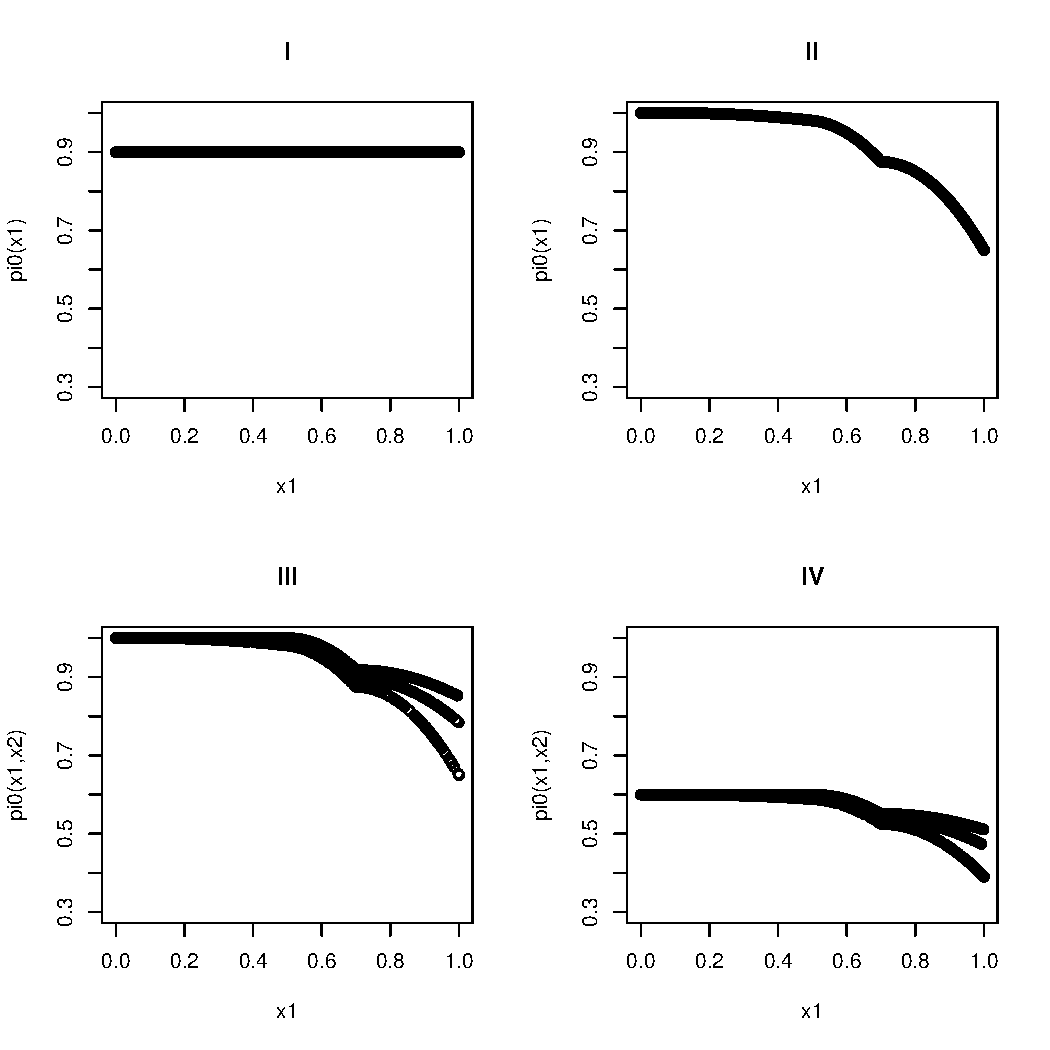
\includegraphics[width=\maxwidth]{Figures/unnamed-chunk-3-1} 

}



\end{knitrout}

\clearpage




  
  Estimated false discovery rates (FDR) and true positive rates (TPR). BL = Boca-Leek. W.S. = well-separated null and alternative, P.S. = poorly separated null and alternative. For III and IV, a dummy variable was used for $x_{2}$, along with linear or spline terms for $x_1$. Used reviewer's definition of "well-separated" and "poorly-separated." Used the theoretical null for the Scott method. For the t-test, considered 2 groups of 6 (so 2x6 = 10 df) and used the t-statistics instead of the z-statistics for the Scott method.
% latex table generated in R 3.3.1 by xtable 1.8-2 package
% Thu Jun 22 11:09:38 2017
\begin{table}[ht]
\centering
\begin{tabular}{lll|llll|llll}
  \hline
  &&& \multicolumn{4}{c}{FDR} & \multicolumn{4}{c}{TPR}\\
 $\pi_0(x)$ &  Distribution under $H_1$ & Regression model & BL & Scott & Storey & BH & BL & Scott & Storey & BH    \\
 \hline
I & Beta(1,20) & Linear & 0.05 & 0.90 & 0.05 & 0.04 & 0.00 & 1.00 & 0.00 & 0.00 \\ 
  II & Beta(1,20) & Linear & 0.05 & 0.93 & 0.05 & 0.04 & 0.00 & 1.00 & 0.00 & 0.00 \\ 
  II & Beta(1,20) & Spline & 0.06 & 0.93 & 0.05 & 0.04 & 0.00 & 1.00 & 0.00 & 0.00 \\ 
  III & Beta(1,20) & Linear & 0.05 & 0.95 & 0.05 & 0.05 & 0.00 & 1.00 & 0.00 & 0.00 \\ 
  III & Beta(1,20) & Spline & 0.06 & 0.95 & 0.05 & 0.05 & 0.00 & 1.00 & 0.00 & 0.00 \\ 
  IV & Beta(1,20) & Linear & 0.06 & 0.57 & 0.05 & 0.03 & 0.12 & 1.00 & 0.05 & 0.00 \\ 
  IV & Beta(1,20) & Spline & 0.08 & 0.57 & 0.05 & 0.03 & 0.15 & 1.00 & 0.05 & 0.00 \\ 
   \hline
I & Norm (W.S.) & Linear & 0.05 & 0.05 & 0.05 & 0.04 & 0.51 & 0.51 & 0.51 & 0.50 \\ 
  II & Norm (W.S.) & Linear & 0.05 & 0.06 & 0.05 & 0.05 & 0.49 & 0.64 & 0.48 & 0.47 \\ 
  II & Norm (W.S.) & Spline & 0.06 & 0.06 & 0.05 & 0.05 & 0.49 & 0.64 & 0.48 & 0.47 \\ 
  III & Norm (W.S.) & Linear & 0.06 & 0.06 & 0.05 & 0.05 & 0.45 & 0.60 & 0.44 & 0.43 \\ 
  III & Norm (W.S.) & Spline & 0.06 & 0.06 & 0.05 & 0.05 & 0.46 & 0.61 & 0.44 & 0.43 \\ 
  IV & Norm (W.S.) & Linear & 0.05 & 0.05 & 0.05 & 0.03 & 0.72 & 0.72 & 0.71 & 0.65 \\ 
  IV & Norm (W.S.) & Spline & 0.05 & 0.05 & 0.05 & 0.03 & 0.72 & 0.72 & 0.71 & 0.65 \\ 
   \hline
I & Norm (P.S.) & Linear & 0.06 & 0.05 & 0.05 & 0.05 & 0.03 & 0.03 & 0.03 & 0.03 \\ 
  II & Norm (P.S.) & Linear & 0.05 & 0.05 & 0.05 & 0.05 & 0.03 & 0.05 & 0.03 & 0.02 \\ 
  II & Norm (P.S.) & Spline & 0.05 & 0.05 & 0.05 & 0.05 & 0.03 & 0.05 & 0.03 & 0.02 \\ 
  III & Norm (P.S.) & Linear & 0.08 & 0.04 & 0.07 & 0.07 & 0.02 & 0.04 & 0.02 & 0.02 \\ 
  III & Norm (P.S.) & Spline & 0.08 & 0.05 & 0.07 & 0.07 & 0.03 & 0.05 & 0.02 & 0.02 \\ 
  IV & Norm (P.S.) & Linear & 0.04 & 0.04 & 0.04 & 0.03 & 0.08 & 0.08 & 0.07 & 0.06 \\ 
  IV & Norm (P.S.) & Spline & 0.04 & 0.04 & 0.04 & 0.03 & 0.08 & 0.08 & 0.07 & 0.06 \\ 
   \hline
I & T (W.S.) & Linear & 0.06 & 0.21 & 0.06 & 0.05 & 0.16 & 0.55 & 0.15 & 0.14 \\ 
  II & T (W.S.) & Linear & 0.05 & 0.21 & 0.05 & 0.04 & 0.13 & 0.64 & 0.12 & 0.11 \\ 
  II & T (W.S.) & Spline & 0.05 & 0.21 & 0.05 & 0.04 & 0.14 & 0.65 & 0.12 & 0.11 \\ 
  III & T (W.S.) & Linear & 0.06 & 0.27 & 0.06 & 0.05 & 0.09 & 0.55 & 0.08 & 0.08 \\ 
  III & T (W.S.) & Spline & 0.07 & 0.27 & 0.06 & 0.05 & 0.10 & 0.55 & 0.08 & 0.08 \\ 
  IV & T (W.S.) & Linear & 0.05 & 0.09 & 0.05 & 0.03 & 0.52 & 0.73 & 0.52 & 0.40 \\ 
  IV & T (W.S.) & Spline & 0.05 & 0.09 & 0.05 & 0.03 & 0.53 & 0.73 & 0.52 & 0.40 \\ 
   \hline
I & T (P.S.) & Linear & 0.08 & 0.46 & 0.08 & 0.08 & 0.00 & 0.08 & 0.00 & 0.00 \\ 
  II & T (P.S.) & Linear & 0.07 & 0.44 & 0.06 & 0.06 & 0.00 & 0.11 & 0.00 & 0.00 \\ 
  II & T (P.S.) & Spline & 0.07 & 0.44 & 0.06 & 0.06 & 0.00 & 0.11 & 0.00 & 0.00 \\ 
  III & T (P.S.) & Linear & 0.08 & 0.60 & 0.08 & 0.08 & 0.00 & 0.08 & 0.00 & 0.00 \\ 
  III & T (P.S.) & Spline & 0.09 & 0.60 & 0.08 & 0.08 & 0.00 & 0.08 & 0.00 & 0.00 \\ 
  IV & T (P.S.) & Linear & 0.04 & 0.15 & 0.03 & 0.03 & 0.01 & 0.14 & 0.01 & 0.00 \\ 
  IV & T (P.S.) & Spline & 0.05 & 0.15 & 0.03 & 0.03 & 0.01 & 0.14 & 0.01 & 0.00 \\ 
   \hline
\end{tabular}
\end{table}


\clearpage

  Estimated false discovery rates (FDR) and true positive rates (TPR). BL = Boca-Leek. W.S. = well-separated null and alternative, P.S. = poorly separated null and alternative. For III and IV, a dummy variable was used for $x_{2}$, along with linear or spline terms for $x_1$. Extended "well-separated" and "poorly-separated" definition to chisquared test, generating means fom the absolute value of a normal distribution with mean 9, respectively 1. For the chisquared test, 1 df corresponds to a 2x2 table, 4 df to a 3x3 table. Used the z-values obtained from back-transforming the p-values for the Scott method in this case.
% latex table generated in R 3.3.1 by xtable 1.8-2 package
% Thu Jun 22 11:09:38 2017
\begin{table}[ht]
\centering
\begin{tabular}{lll|llll|llll}
  \hline
  &&& \multicolumn{4}{c}{FDR} & \multicolumn{4}{c}{TPR}\\
 $\pi_0(x)$ &  Distribution under $H_1$ & Regression model & BL & Scott & Storey & BH & BL & Scott & Storey & BH    \\
 \hline
I & Chisq 1 df (W.S.) & Linear & 0.05 & 0.90 & 0.05 & 0.04 & 0.51 & 1.00 & 0.51 & 0.50 \\ 
  II & Chisq 1 df (W.S.) & Linear & 0.05 & 0.93 & 0.05 & 0.04 & 0.48 & 1.00 & 0.47 & 0.46 \\ 
  II & Chisq 1 df (W.S.) & Spline & 0.05 & 0.93 & 0.05 & 0.04 & 0.49 & 1.00 & 0.47 & 0.46 \\ 
  III & Chisq 1 df (W.S.) & Linear & 0.05 & 0.95 & 0.05 & 0.05 & 0.44 & 1.00 & 0.43 & 0.42 \\ 
  III & Chisq 1 df (W.S.) & Spline & 0.05 & 0.95 & 0.05 & 0.05 & 0.45 & 1.00 & 0.43 & 0.42 \\ 
  IV & Chisq 1 df (W.S.) & Linear & 0.05 & 0.57 & 0.05 & 0.03 & 0.72 & 1.00 & 0.71 & 0.65 \\ 
  IV & Chisq 1 df (W.S.) & Spline & 0.05 & 0.57 & 0.05 & 0.03 & 0.72 & 1.00 & 0.71 & 0.65 \\ 
   \hline
I & Chisq 4 df (W.S.) & Linear & 0.05 & 0.90 & 0.05 & 0.05 & 0.31 & 1.00 & 0.31 & 0.30 \\ 
  II & Chisq 4 df (W.S.) & Linear & 0.05 & 0.93 & 0.05 & 0.05 & 0.28 & 1.00 & 0.28 & 0.27 \\ 
  II & Chisq 4 df (W.S.) & Spline & 0.05 & 0.93 & 0.05 & 0.05 & 0.29 & 1.00 & 0.28 & 0.27 \\ 
  III & Chisq 4 df (W.S.) & Linear & 0.06 & 0.95 & 0.05 & 0.05 & 0.25 & 1.00 & 0.24 & 0.23 \\ 
  III & Chisq 4 df (W.S.) & Spline & 0.06 & 0.95 & 0.05 & 0.05 & 0.25 & 1.00 & 0.24 & 0.23 \\ 
  IV & Chisq 4 df (W.S.) & Linear & 0.05 & 0.57 & 0.05 & 0.03 & 0.52 & 1.00 & 0.52 & 0.45 \\ 
  IV & Chisq 4 df (W.S.) & Spline & 0.05 & 0.57 & 0.05 & 0.03 & 0.53 & 1.00 & 0.52 & 0.45 \\ 
   \hline
I & Chisq 1 df (P.S.) & Linear & 0.04 & 0.90 & 0.04 & 0.03 & 0.03 & 1.00 & 0.03 & 0.03 \\ 
  II & Chisq 1 df (P.S.) & Linear & 0.06 & 0.93 & 0.05 & 0.05 & 0.02 & 1.00 & 0.02 & 0.02 \\ 
  II & Chisq 1 df (P.S.) & Spline & 0.06 & 0.93 & 0.05 & 0.05 & 0.02 & 1.00 & 0.02 & 0.02 \\ 
  III & Chisq 1 df (P.S.) & Linear & 0.05 & 0.95 & 0.04 & 0.04 & 0.02 & 1.00 & 0.02 & 0.02 \\ 
  III & Chisq 1 df (P.S.) & Spline & 0.05 & 0.95 & 0.04 & 0.04 & 0.02 & 1.00 & 0.02 & 0.02 \\ 
  IV & Chisq 1 df (P.S.) & Linear & 0.04 & 0.57 & 0.03 & 0.03 & 0.07 & 1.00 & 0.07 & 0.06 \\ 
  IV & Chisq 1 df (P.S.) & Spline & 0.04 & 0.57 & 0.03 & 0.03 & 0.08 & 1.00 & 0.07 & 0.06 \\ 
   \hline
I & Chisq 4 df (P.S.) & Linear & 0.07 & 0.90 & 0.06 & 0.06 & 0.01 & 1.00 & 0.01 & 0.01 \\ 
  II & Chisq 4 df (P.S.) & Linear & 0.05 & 0.93 & 0.05 & 0.05 & 0.01 & 1.00 & 0.01 & 0.01 \\ 
  II & Chisq 4 df (P.S.) & Spline & 0.05 & 0.93 & 0.05 & 0.05 & 0.01 & 1.00 & 0.01 & 0.01 \\ 
  III & Chisq 4 df (P.S.) & Linear & 0.06 & 0.95 & 0.06 & 0.06 & 0.01 & 1.00 & 0.01 & 0.01 \\ 
  III & Chisq 4 df (P.S.) & Spline & 0.07 & 0.95 & 0.06 & 0.06 & 0.01 & 1.00 & 0.01 & 0.01 \\ 
  IV & Chisq 4 df (P.S.) & Linear & 0.05 & 0.57 & 0.05 & 0.04 & 0.02 & 1.00 & 0.02 & 0.01 \\ 
  IV & Chisq 4 df (P.S.) & Spline & 0.05 & 0.57 & 0.05 & 0.04 & 0.02 & 1.00 & 0.02 & 0.01 \\ 
   \hline
\end{tabular}
\end{table}


\end{document}
